%%%%%%%%%%%%%%%%%%%%%%%%%%%%%%%%%%%%%%%%%
% Beamer Presentation
% LaTeX Template
% Version 1.0 (10/11/12)
%
% This template has been downloaded from:
% http://www.LaTeXTemplates.com
%
% License:
% CC BY-NC-SA 3.0 (http://creativecommons.org/licenses/by-nc-sa/3.0/)
%
%%%%%%%%%%%%%%%%%%%%%%%%%%%%%%%%%%%%%%%%%

%----------------------------------------------------------------------------------------
%	PACKAGES AND THEMES
%----------------------------------------------------------------------------------------

% \documentclass[12pt, french]{article}

\documentclass[french]{beamer}

\usepackage[utf8]{inputenc}
\usepackage[T1]{fontenc}
\usepackage{babel}

\mode<presentation> {

% The Beamer class comes with a number of default slide themes
% which change the colors and layouts of slides. Below this is a list
% of all the themes, uncomment each in turn to see what they look like.

%\usetheme{default}
%\usetheme{AnnArbor}
%\usetheme{Antibes}
%\usetheme{Bergen}
%\usetheme{Berkeley}
%\usetheme{Berlin}
%\usetheme{Boadilla}
%\usetheme{CambridgeUS}
%\usetheme{Copenhagen}
%\usetheme{Darmstadt}
%\usetheme{Dresden}
%\usetheme{Frankfurt}
%\usetheme{Goettingen}
%\usetheme{Hannover}
%\usetheme{Ilmenau}
%\usetheme{JuanLesPins}
%\usetheme{Luebeck}
\usetheme{Madrid}
%\usetheme{Malmoe}
%\usetheme{Marburg}
%\usetheme{Montpellier}
%\usetheme{PaloAlto}
%\usetheme{Pittsburgh}
%\usetheme{Rochester}
%\usetheme{Singapore}
%\usetheme{Szeged}
%\usetheme{Warsaw}

% As well as themes, the Beamer class has a number of color themes
% for any slide theme. Uncomment each of these in turn to see how it
% changes the colors of your current slide theme.

%\usecolortheme{albatross}
%\usecolortheme{beaver}
%\usecolortheme{beetle}
%\usecolortheme{crane}
%\usecolortheme{dolphin}
%\usecolortheme{dove}
%\usecolortheme{fly}
%\usecolortheme{lily}
%\usecolortheme{orchid}
%\usecolortheme{rose}
%\usecolortheme{seagull}
%\usecolortheme{seahorse}
%\usecolortheme{whale}
%\usecolortheme{wolverine}

%\setbeamertemplate{footline} % To remove the footer line in all slides uncomment this line
%\setbeamertemplate{footline}[page number] % To replace the footer line in all slides with a simple slide count uncomment this line

%\setbeamertemplate{navigation symbols}{} % To remove the navigation symbols from the bottom of all slides uncomment this line
}

\usepackage{graphicx} % Allows including images
\usepackage{booktabs} % Allows the use of \toprule, \midrule and \bottomrule in tables

\usepackage{tikz}
\usetikzlibrary{calc,decorations.markings}

\usetikzlibrary{arrows}

\usepackage{tkz-graph}
% \GraphInit[vstyle = Shade]
\tikzset{
	LabelStyle/.style = { rectangle, rounded corners, draw,
		minimum width = 2em, fill = yellow!50,
		text = red, font = \bfseries },
	VertexStyle/.append style = { inner sep=5pt,
		font = \Large\bfseries},
	%	EdgeStyle/.append style = {->, bend left} % by default graphs are non-oriented. Individually: put this line on to make them oriented.
}

\tikzset{
	treenode/.style = {align=center, inner sep=0pt, text centered,
		font=\sffamily},
	arn_n/.style = {treenode, circle, black, font=\sffamily\bfseries, draw=black,
		fill=white, text width=2em},% arbre rouge noir, noeud noir
	arn_r/.style = {treenode, circle, red, draw=red, 
		text width=1.5em, very thick},% arbre rouge noir, noeud rouge
	arn_x/.style = {treenode, rectangle, draw=black,
		minimum width=0.5em, minimum height=0.5em}% arbre rouge noir, nil
}

\usepackage{dingbat}

\newcommand{\states}{\ensuremath{\big.{S}}}
\newcommand{\actions}{\ensuremath{\big.{A}}}

%----------------------------------------------------------------------------------------
%	TITLE PAGE
%----------------------------------------------------------------------------------------

\title[Parcours, Août 2018]{Parcours} % The short title appears at the bottom of every slide, the full title is only on the title page
\subtitle{On en est où?}

\author{Équipe TESD} % Your name
\institute[CRIM] % Your institution as it will appear on the bottom of every slide, may be shorthand to save space
{
CRIM \\ % Your institution for the title page
\medskip
\textit{prenom.nom@crim.ca} % Your email address
}
\date{31 Août 2018} % Date, can be changed to a custom date

\begin{document}

\begin{frame}
\titlepage % Print the title page as the first slide
\end{frame}

% \begin{frame}
% \frametitle{Overview} % Table of contents slide, comment this block out to remove it
% \tableofcontents % Throughout your presentation, if you choose to use \section{} and \subsection{} commands, these will automatically be printed on this slide as an overview of your presentation
% \end{frame}

%----------------------------------------------------------------------------------------
%	PRESENTATION SLIDES
%----------------------------------------------------------------------------------------

%------------------------------------------------
\section{Main} % Sections can be created in order to organize your presentation into discrete blocks, all sections and subsections are automatically printed in the table of contents as an overview of the talk
%------------------------------------------------

\subsection{Main} % A subsection can be created just before a set of slides with a common theme to further break down your presentation into chunks


\begin{frame}
\frametitle{Définition du Problème}

	\begin{itemize}
		\item VdM: améliorer l'efficacité opérationnelle des parcours des véhicule+ minimiser l'impact de leur déplacement. 
			\begin{itemize}
				\item découpage du territoire
				\item couverture optimale du territoire
			\end{itemize}
		\item modélisation: problèmes réels $\Longrightarrow$ problèmes de tournées de véhicules
			\begin{itemize}
				\item Demandes sur les nœuds? VRPs!
				\item Demandes sur les arcs? ARPs!
			\end{itemize}
	\end{itemize}

%\begin{figure}[!htb]
%	\centering

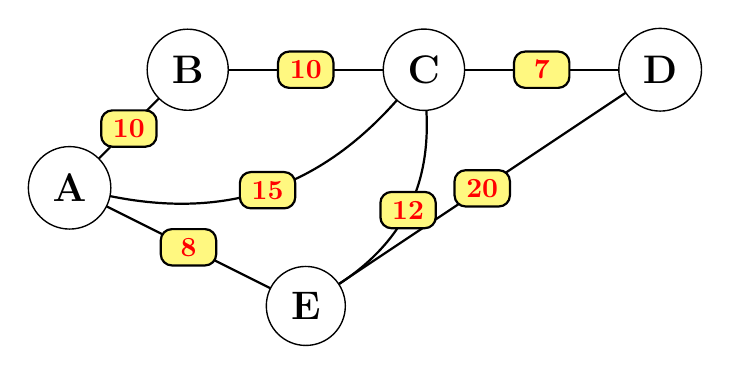
\begin{tikzpicture}[scale=0.750]
\SetGraphUnit{5}
\Vertex{A}
\Vertex[x=2,y=2]{B}
\Vertex[x=6,y=2]{C}
\Vertex[x=10,y=2]{D}
\Vertex[x=4,y=-2]{E}
\Edge[label = 10](A)(B)
\Edge[label = 10](B)(C)
\Edge[label = 7](C)(D)
\Edge[label = 20](D)(E)
\Edge[label = 8](E)(A)
\tikzset{
	EdgeStyle/.append style = {bend left} 
}
\Edge[label = 12](C)(E)
\Edge[label = 15](C)(A)
\tikzset{
	EdgeStyle/.append style = {bend right} 
}
% \Edge[label = 14](B)(E)
\end{tikzpicture}
%\end{figure}

\end{frame}

%------------------------------------------------

\begin{frame}
\frametitle{On en est où?}

\begin{block}{En général: problème est un ARP: bibliographie}
	\begin{itemize}
		\item Algorithmes? \checkmark
		\item Sectorisation? \checkmark
		\item Modèles de données? \checkmark
	\end{itemize}
\end{block}

\begin{block}{VdM (I): Sectorisation}
	Proposition de combinaison de mesures pour modéliser une grande gamme de problèmes. 
	Mesures de base:
	\begin{itemize}
		\item Équilibre
		\item Adjacence
		\item Compacité
		\item Désirabilité
	\end{itemize}
\end{block}


\end{frame}

%------------------------------------------------

\begin{frame}
\frametitle{On en est où? (ct'd)}

\begin{block}{VdM (II): Modèles de Données}
	Étude de différents modèles, impressions sur page Excel. 
	
	Spécification de nos besoins:
	\begin{enumerate}
		\item Pour chaque route (arc): quelles sont les voies qui y circulent, incluant la forme et la limite de vitesse de chacune.
		\item Sur les intersections:
		\begin{enumerate}
			\item Leur géo-localisation.
			\item La logique des feux de circulation.
			\item La priorité des véhicules qu s'y engagent.
		\end{enumerate}
		\item Districts.
		\item Descriptions des rond-points.
	\end{enumerate}
	+ d'un format XML pour communication.
\end{block}


\end{frame}

%------------------------------------------------


%------------------------------------------------

\begin{frame}
\Huge{\centerline{The End}}
\end{frame}

%----------------------------------------------------------------------------------------

\end{document}